% !TEX root =  master.tex
\chapter{DART}

Als Videoquelle dient der Löwen-DART HB10, dieser erstellt kurze Videoschnipsel für jeden Wurf, aus einem Spiel des Zukünftigen Turnier Modus. Nach Abschluss des Spiels werden alle Videoschnipsel zu einem Video zusammengeführt, und für das Streaming vorbereitet. 

\section{Aufbau und Ablauf}

Die Videofunktion des HB10 erstreckt sich über zwei Anwendungen, welche miteinander kommunizieren. Die erste ist die eigentliche DART-Anwendung, diese ist dafür zuständig die zweite Anwendung über Ereignisse wie Treffer, Spiel Start und Ende zu Informieren,
sowie das Abschließende übertragen an den Server. Die zweite Anwendung, ist verantwortlich für das zwischen Speichern, das Zusammenschneiden, das Komprimieren der Videodaten, sowie das anschließende erstellen der Playlist.

\subsection{Ablauf}

\subsubsection{Verarbeitung eines Wurfes bis zur Bereitstellung des Videos}

Das erste Sequenzdiagramm beschreibt den fachlichen Hauptablauf zwischen \texttt{Dart\_App}, \texttt{Video\_Main}, \texttt{File\_System} und \texttt{Server}. Im Zentrum steht dabei die ereignisgesteuerte Verarbeitung eines Dartwurfs sowie die nachgelagerte Aufbereitung der Videodaten nach Spielende. 
Der \texttt{VideoHandler} empfängt die von der Anwendung gesendeten Nachrichten als \texttt{VideoQuery}-Objekte, wobei insbesondere die Kommandos \texttt{DART\_HIT} und \texttt{GAME\_END} für diesen Ablauf relevant sind.

\begin{figure}[H]
    \centering
    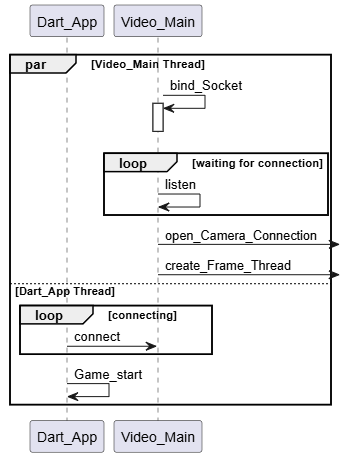
\includegraphics[width=0.55\textwidth]{img/PlantUml/DartSequenz1.png}
    \caption{Ablauf vom registrierten Dartwurf bis zur Bereitstellung des verarbeiteten Videos}
    \label{fig:dartsequenz1}
\end{figure}

Während das Spiel noch läuft, sendet die \texttt{Dart\_App} bei einem erkannten Treffer das Ereignis \texttt{send\_Hit} an \texttt{Video\_Main}. Im Quellcode entspricht dies dem Empfang eines \texttt{VideoQuery}-Objekts mit dem Kommando \texttt{DART\_HIT}. 
Nach der Deserialisierung der Nachricht wird der jeweilige Spieler über die \texttt{playerId} identifiziert und in die Menge der aktiven Spieler aufgenommen. Anschließend wird eine kurze Verzögerung von 1{,}5 Sekunden eingehalten, 
damit zusätzlich auch die unmittelbar nach dem Treffer aufgenommenen Frames in die zugehörige Videosequenz einfließen können.
Die Grundlage dafür bildet ein Ringpuffer, der kontinuierlich mit Kameradaten gefüllt wird. Dieser Puffer besitzt eine Größe von \texttt{fps * seconds} und enthält damit bei der aktuellen Konfiguration drei Sekunden Rohvideodaten mit zehn Bildern pro Sekunde. Sobald ein Treffer verarbeitet wird, 
wird eine Kopie des Puffers erstellt und ausgehend von der aktuellen Pufferposition in die chronologisch korrekte Reihenfolge gebracht. Die so gesicherten Frames werden anschließend als rohe \texttt{.yuv}-Datei im spielerspezifischen Verzeichnis unter 
\texttt{/media/nfs\_vdai/<playerId>/throw<throwId>.yuv} abgelegt. Wenn es sich um den ersten Wurf eines Spiels handelt, wird das bisherige Spielerverzeichnis zuvor gelöscht und anschließend neu angelegt. 

Der zweite Teil des Diagramms zeigt den Ablauf nach Spielende. Sobald \texttt{Dart\_App} das Signal \texttt{send\_game\_finished} sendet, verarbeitet \texttt{Video\_Main} im \texttt{VideoHandler} das Kommando \texttt{GAME\_END}. 
Für jeden aktiven Spieler werden nun sämtliche zuvor gespeicherten Rohdateien aus dem Dateisystem eingelesen. Dabei werden die einzelnen Dateien sortiert verarbeitet, damit die daraus entstehende Gesamtsequenz der zeitlichen Reihenfolge der Würfe entspricht. 

Im Anschluss erfolgt die eigentliche Videonachbearbeitung. Die eingelesenen Rohdaten liegen zunächst im Format \texttt{YUYV422} vor und werden über \texttt{convertYUYVtoYUV420P} in das für die softwarebasierte Kodierung benötigte Format \texttt{YUV420P} überführt. 
Danach komprimiert \texttt{compressVideosSw} die Bildfolge mit dem Encoder \texttt{libopenh264} zu einer MP4-Datei. Diese Datei wird im Spielerverzeichnis als \texttt{game.mp4} gespeichert. Anschließend erzeugt \texttt{createHlsPlaylist} aus dieser MP4-Datei eine HLS-Wiedergabestruktur mit einer 
\texttt{playlist.m3u8} sowie segmentierten \texttt{.ts}-Dateien. Die Segmentlänge ist dabei auf ungefähr vier Sekunden konfiguriert. 

Zum Abschluss wird das Ergebnis an die \texttt{Dart\_App} zurückgemeldet. Hierzu erstellt der \texttt{VideoHandler} ein \texttt{VideoReply}-Objekt, in dem die Anzahl der erzeugten Videos sowie zusätzliche Pfadinformationen gespeichert werden. Die Antwort enthält für 
jeden verarbeiteten Spieler den Pfad zur erzeugten Videostruktur und die Anzahl der HLS-Segmente. Dieses Verhalten entspricht im Diagramm der Rückmeldung \texttt{send\_video\_finished(path)}, dem anschließenden Abruf des Videos und dem finalen Upload zum \texttt{Server}. 
Insgesamt verdeutlicht das erste Diagramm damit die Trennung zwischen einer leichtgewichtigen Rohdatenspeicherung während des Spiels und der rechenintensiven Aufbereitung nach Spielende.

\subsubsection{Initialisierung des Video-Subsystems und Verbindungsaufbau}

Das zweite Sequenzdiagramm fokussiert die Initialisierung des Systems und zeigt, dass sich der Gesamtablauf aus zwei parallel angelegten Teilschritten zusammensetzt: dem Thread von \texttt{Video\_Main} und dem Thread der \texttt{Dart\_App}. Ziel dieser Startphase ist es, 
zunächst die Kommunikationsverbindung zwischen beiden Komponenten herzustellen und danach die Kameraverbindung für die kontinuierliche Videoaufnahme zu initialisieren.

\begin{figure}[H]
    \centering
    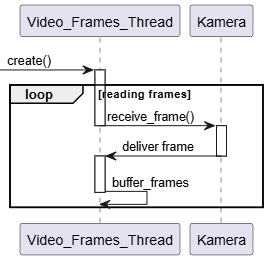
\includegraphics[width=0.5\textwidth]{img/PlantUml/DartSequenz2.png}
    \caption{Initialisierung von Socket-Kommunikation und Kameraverbindung}
    \label{fig:dartsequenz2}
\end{figure}

Auf Seiten von \texttt{Video\_Main} beginnt der Ablauf mit der Initialisierung im \texttt{VideoHandler::init()}. Dabei wird zunächst der interne Videopuffer vorbereitet, dessen Größe sich aus Bildrate, Aufzeichnungsdauer sowie der gewählten Auflösung ergibt. 
Anschließend wird über \texttt{getaddrinfo()}, \texttt{socket()}, \texttt{bind()} und \texttt{listen()} ein TCP-Server auf der lokalen Adresse \texttt{127.0.0.1} und dem Port \texttt{56970} eingerichtet. Nachdem der Socket erfolgreich gebunden wurde, wechselt das System in einen Wartezustand, 
in dem eingehende Verbindungen mit \texttt{accept()} entgegengenommen werden. Genau dieser Zustand wird im Diagramm durch die Schleife \texttt{[waiting for connection]} dargestellt.

Parallel dazu versucht die \texttt{Dart\_App}, eine Verbindung zum bereitgestellten Socket aufzubauen. Im Diagramm ist dies als Schleife \texttt{[connecting]} mit dem Aufruf \texttt{connect} dargestellt. Sobald die Verbindung erfolgreich hergestellt wurde,
protokolliert der \texttt{VideoHandler} den erfolgreichen Verbindungsaufbau und setzt die weitere Initialisierung fort. Damit ist die Kommunikationsgrundlage geschaffen, über die im späteren Spielverlauf Ereignisse wie \texttt{DART\_HIT} oder \texttt{GAME\_END} übertragen werden.

Nach erfolgreicher Socket-Verbindung initialisiert \texttt{Video\_Main} die Kameraschnittstelle. Dies geschieht über \texttt{findStream()}, wobei FFmpeg zunächst für Eingabegeräte registriert wird und danach ein V4L2-Eingabestream für \texttt{/dev/video0} geöffnet wird. 
Zusätzlich werden dabei die Aufnahmeparameter gesetzt, insbesondere die Auflösung von \texttt{1280 x 720}, die Bildrate von \texttt{10} Bildern pro Sekunde und das Eingabeformat \texttt{yuyv422}. 
Im Diagramm wird dieser Abschnitt durch die Aktionen \texttt{open\_Camera\_Connection} und \texttt{create\_Frame\_Thread} abstrahiert.

Sobald der Kamerastream erfolgreich geöffnet wurde, startet der \texttt{VideoHandler} einen separaten Thread zur Frame-Erfassung. Dieser Schritt ist wesentlich, weil dadurch die Netzwerkkommunikation und die Aufnahme der Videodaten voneinander entkoppelt werden. 
Die \texttt{Dart\_App} signalisiert anschließend mit \texttt{Game\_start} den eigentlichen Beginn des Spielbetriebs. Das zweite Diagramm macht damit deutlich, dass die Videoverarbeitung nicht erst beim ersten Wurf beginnt, sondern bereits vorher vollständig initialisiert sein muss, 
damit Trefferereignisse ohne Verzögerung verarbeitet werden können. 

\subsubsection{Kontinuierliche Erfassung und Pufferung der Kameraframes}

Das dritte Sequenzdiagramm zeigt den technischen Kern der laufenden Aufnahme, nämlich die kontinuierliche Erfassung der Kameraframes in einem dedizierten Thread. Dieser Thread ist im \texttt{VideoHandler} als \texttt{frameLoop} umgesetzt und führt die Funktion \texttt{readingFrameLoop()} aus. 
Das Diagramm konzentriert sich damit nicht auf die fachlichen Spielereignisse, sondern auf den fortlaufenden Datenstrom zwischen der Kamera und dem internen Pufferspeicher.

\begin{figure}[H]
    \centering
    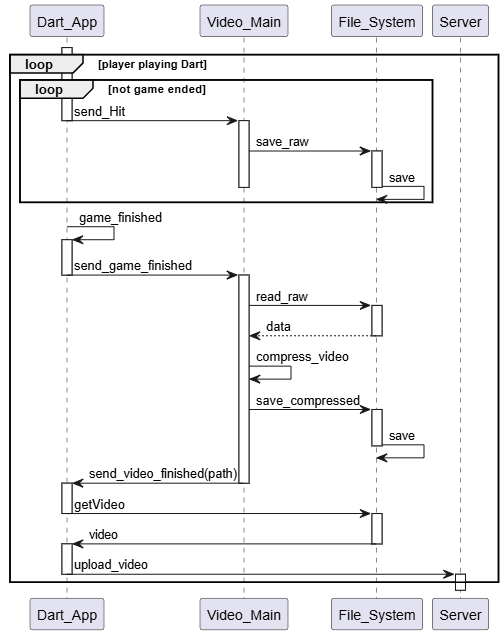
\includegraphics[width=0.65\textwidth]{img/PlantUml/DartSequenz3.png}
    \caption{Kontinuierliche Erfassung und Zwischenspeicherung von Kameraframes}
    \label{fig:dartsequenz3}
\end{figure}

Zu Beginn wird der Thread erzeugt, nachdem die Kameraverbindung erfolgreich initialisiert wurde. Innerhalb von \texttt{readingFrameLoop()} wird zunächst ein \texttt{AVPacket} reserviert; anschließend läuft eine Schleife, die so lange aktiv bleibt, wie der \texttt{VideoHandler} insgesamt aktiv ist. 
Innerhalb dieser Schleife werden fortlaufend Frames über \texttt{readFrame()} von der Kamera gelesen. Dieser Ablauf entspricht im Diagramm der wiederholten Interaktion \texttt{receive\_frame()} zwischen \texttt{Video\_Frames\_Thread} und \texttt{Kamera}.

Wenn ein gültiges Videopaket empfangen wurde, wird dessen Inhalt in den internen \texttt{videoBuffer} übernommen. Der Puffer ist als Ringstruktur realisiert: Nach jedem gespeicherten Frame wird der Index erhöht, und sobald das Ende des Puffers erreicht ist, springt der Index wieder auf den Anfang zurück. 
Dadurch enthält der Puffer zu jedem Zeitpunkt stets die zuletzt aufgenommenen Frames. Das Diagramm stellt diesen Schritt durch die Aktionen \texttt{deliver frame} und \texttt{buffer\_frames} dar.

Diese Pufferlogik ist entscheidend für die spätere Verarbeitung eines Darttreffers. Da beim Eintreffen eines \texttt{DART\_HIT}-Ereignisses nicht erst eine neue Aufnahme gestartet wird, sondern auf bereits vorhandene Bilddaten zurückgegriffen wird,
kann auch der zeitliche Kontext unmittelbar vor dem Treffer rekonstruiert werden. Zusammen mit der im Trefferfall eingebauten Nachlaufzeit entsteht so pro Wurf eine kurze, aber vollständige Videosequenz. Das dritte Diagramm erläutert somit die technische Voraussetzung dafür, 
dass das im ersten Diagramm dargestellte Speichern einzelner Wurfsequenzen überhaupt möglich ist.

Zusammengenommen zeigen die drei Diagramme einen durchgängigen Gesamtprozess: Das zweite Diagramm beschreibt die Initialisierung der Kommunikation und der Kamera, das dritte Diagramm die kontinuierliche Erfassung und Zwischenspeicherung der Frames und das erste Diagramm 
schließlich die fachliche Verarbeitung der Spielereignisse bis zur Erzeugung und Bereitstellung der finalen Videos. Die Aufteilung in diese drei Sichten erleichtert das Verständnis, weil Initialisierung, Laufzeitverhalten und Nachverarbeitung jeweils getrennt, 
zugleich aber konsistent innerhalb derselben \texttt{VideoHandler}-Architektur dargestellt werden.

\newpage